\documentclass[]{llncs} 
\usepackage{tikz} 
\usepackage{verbatim}

\author{Valentin Mayer-Eichberger}

\institute{IVU Traffice Technologies\\ Bundesallee 88, 12000 Berlin\\
\email{vme@ivu.de}}

\title{ASP Encodings of Spinpossible}

\newcommand{\code}[1]{\verb|#1|} 
\newcommand{\spintable}[9]{ 
\node [matrix,ampersand replacement=\&,nodes={minimum size=4mm}]
%,nodes={fill=blue!20,minimum size=5mm}] 
{
    \node {#1}; \& \node{#2}; \& \node {#3}; \\ 
    \node {#4}; \& \node{#5}; \& \node {#6}; \\ 
    \node {#7}; \& \node{#8}; \& \node {#9}; \\ 
}; 
}

\begin{document} \maketitle

\section{ASP encoding}



\subsection{Motivation for vector representation}

The two following problems are essentially the same. Replacing $-8$ with $1$ in the
first and $3$ and $-4$ in the second requires the same kind of spins. 

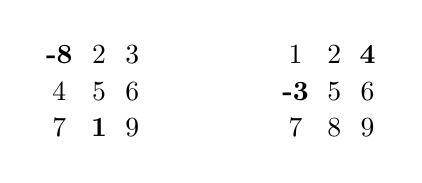
\begin{tikzpicture} 
\spintable{\textbf{-8}}{2}{3}{4}{5}{6}{7}{\textbf{1}}{9}
\begin{scope}[xshift=3cm] 
\spintable{1}{2}{\textbf{4}}{\textbf{-3}}{5}{6}{7}{8}{9}
\end{scope} 
\end{tikzpicture}

Human players detect that instantely. We will explain in following two paragraphs how
to arrive at a representation such that these two board and the neccessary spins to
solve them, are the same. 

\paragraph{Vector representation: } First we choose a different representation of the
numbers on the boards. Each number is replaced by the vector pointing to where it
should go, and the parity bit (if the number is upside down its 1, otherwise 0)

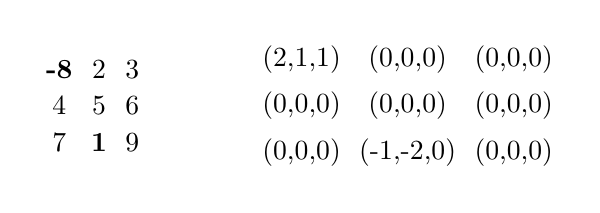
\begin{tikzpicture} 
\spintable{\textbf{-8}}{2}{3}{4}{5}{6}{7}{\textbf{1}}{9}
\begin{scope}[xshift=4cm]
\spintable{(2,1,1)}{(0,0,0)}{(0,0,0)}{(0,0,0)}{(0,0,0)}{(0,0,0)}{(0,0,0)}{(-1,-2,0)}{(0,0,0)}
\end{scope} 
\end{tikzpicture}

E.g. the number in the upper left has to go down by two and one to the right. 


\paragraph{Order on states: } To further unify the two initial boards we need to
define an ordering such that we rotate and reflect the rectangle to a canonical
representation. Lets view the board as a vector of n numbers, e.g. the first board
would be $(-8,2,3,4,5,6,7,1,9)$, or in the vector representation 
\[
((2,1,1),(0,0,0),(0,0,0),(0,0,0),(0,0,0),(0,0,0),(0,0,0),(-1,-2,0),(0,0,0)) 
\] 
Let the ordering $<_{lex}$ be the lexicographic ordering on the vector representation.

For a board there are 8 symmetric representation, generated by $id$,$90°$,
reflection, and combinations of these. 

To find the canonical representation for a board is then to find the maximal element
under the lexicographic ordering $<_{lex}$ among all possible symmetric translations
of the board.

It remains to be shown that the overhead of estimating the correct turn and changing
the board justifies the decrease in visited nodes.  The basic idea is that the
computed nogoods have a wider usage throught the search tree.

\paragraph{Fixing boarder rows/columns: } The two boards from the motivation are now
quite similar, but still not the same. To find the ultimative canonical
representation we need to realize that the side column what is not used by the spins
to solve such a board is not needed and can be omited. This still has to be proven
...

If we remove the unused columns and rows before estimating the maximal element of the
symmetric translations the boards should finally be the same. This also means that
throughout the search the board decreases in size as we fix more and more rows and
columns. 


\paragraph{Decrease in state variables: } Let the size of the board be $m\cdot n$. In
this paragraph we will omit the move $k$. With a direct approach, to encode $m*n$
numbers with parity in $m*n$ positions requires $2*m^2\cdot n^2$ variables.
\begin{verbatim} 
state(X,Y,V) :- m(X), n(Y), mn(V). % n*m*n*m*2 
\end{verbatim} 
By using the vector representation we can break down the board into each dimension
(x-axis, y-axis, parity), e.g.: 

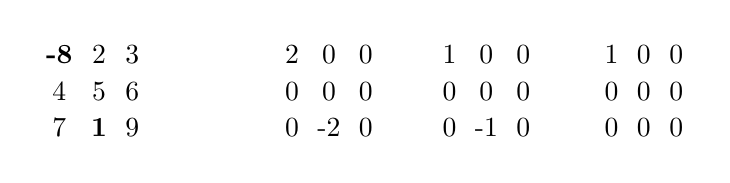
\begin{tikzpicture} 
\spintable{\textbf{-8}}{2}{3}{4}{5}{6}{7}{\textbf{1}}{9}
\begin{scope}[xshift=3cm] 
\spintable{2}{0}{0}{0}{0}{0}{0}{-2}{0} 
\end{scope}
\begin{scope}[xshift=5cm] 
\spintable{1}{0}{0}{0}{0}{0}{0}{-1}{0} 
\end{scope}
\begin{scope}[xshift=7cm] 
\spintable{1}{0}{0}{0}{0}{0}{0}{0}{0} 
\end{scope}
\end{tikzpicture}

representing these three boards as state variables we need the following predicates

\begin{verbatim} 
state(x,X,Y,V) :- m(X), n(Y), m(V). %n*m*m 
state(y,X,Y,V) :- m(X), n(Y), n(V). %n*m*n 
parity(X,Y) :- m(X), n(Y).  %n*m 
\end{verbatim}

These are in total $n*m*(n+m)$ variables!

\subsection{Motivation for recursive state update}

What do the following problems have in common? 

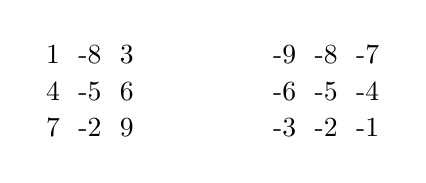
\begin{tikzpicture} 
\spintable{1}{-8}{3}{4}{-5}{6}{7}{-2}{9}
\begin{scope}[xshift=3cm] 
\spintable{-9}{-8}{-7}{-6}{-5}{-4}{-3}{-2}{-1} 
\end{scope}
\end{tikzpicture}

Both can be solved in one step. With spin $(1,0)$ to $(1,2)$ for the first and spin
$(0,0)$ to $(2,2)$ for the second.  But they have more in common: the middle column
switches the same cells. This means the switches of the first spin are implied by the
second spin. How do we use that in our encoding?

Using the breakdown of dimensions we encode a move just in one dimension (omiting
step number and dimension):

\begin{verbatim} 
switch(A+1,B-1) :- switch(A,B),A < B.   % (n^2+n)/2 
\end{verbatim}

Thus a state update is then 


\subsection{State update} State update in dimension $x$ is as follows:

\begin{verbatim} 
state(K+1,x,X2,Y2,X1-X2+V) :-  % k*m^3*n^4 
       state(K,x,X1,Y1,V),
       switch(K+1,x,X1,X2), 
       switch(K+1,y,Y1,Y2).  
\end{verbatim}


\end{document}
